% Options for packages loaded elsewhere
\PassOptionsToPackage{unicode}{hyperref}
\PassOptionsToPackage{hyphens}{url}
%
\documentclass[
  11pt,
  a4paper,
]{article}
\usepackage{amsmath,amssymb}
\usepackage{lmodern}
\usepackage{iftex}
\ifPDFTeX
  \usepackage[T1]{fontenc}
  \usepackage[utf8]{inputenc}
  \usepackage{textcomp} % provide euro and other symbols
\else % if luatex or xetex
  \usepackage{unicode-math}
  \defaultfontfeatures{Scale=MatchLowercase}
  \defaultfontfeatures[\rmfamily]{Ligatures=TeX,Scale=1}
\fi
% Use upquote if available, for straight quotes in verbatim environments
\IfFileExists{upquote.sty}{\usepackage{upquote}}{}
\IfFileExists{microtype.sty}{% use microtype if available
  \usepackage[]{microtype}
  \UseMicrotypeSet[protrusion]{basicmath} % disable protrusion for tt fonts
}{}
\makeatletter
\@ifundefined{KOMAClassName}{% if non-KOMA class
  \IfFileExists{parskip.sty}{%
    \usepackage{parskip}
  }{% else
    \setlength{\parindent}{0pt}
    \setlength{\parskip}{6pt plus 2pt minus 1pt}}
}{% if KOMA class
  \KOMAoptions{parskip=half}}
\makeatother
\usepackage{xcolor}
\usepackage[top=1.5cm, bottom=2cm, left=1.5cm, right=1.5cm]{geometry}
\usepackage{color}
\usepackage{fancyvrb}
\newcommand{\VerbBar}{|}
\newcommand{\VERB}{\Verb[commandchars=\\\{\}]}
\DefineVerbatimEnvironment{Highlighting}{Verbatim}{commandchars=\\\{\}}
% Add ',fontsize=\small' for more characters per line
\usepackage{framed}
\definecolor{shadecolor}{RGB}{248,248,248}
\newenvironment{Shaded}{\begin{snugshade}}{\end{snugshade}}
\newcommand{\AlertTok}[1]{\textcolor[rgb]{0.94,0.16,0.16}{#1}}
\newcommand{\AnnotationTok}[1]{\textcolor[rgb]{0.56,0.35,0.01}{\textbf{\textit{#1}}}}
\newcommand{\AttributeTok}[1]{\textcolor[rgb]{0.77,0.63,0.00}{#1}}
\newcommand{\BaseNTok}[1]{\textcolor[rgb]{0.00,0.00,0.81}{#1}}
\newcommand{\BuiltInTok}[1]{#1}
\newcommand{\CharTok}[1]{\textcolor[rgb]{0.31,0.60,0.02}{#1}}
\newcommand{\CommentTok}[1]{\textcolor[rgb]{0.56,0.35,0.01}{\textit{#1}}}
\newcommand{\CommentVarTok}[1]{\textcolor[rgb]{0.56,0.35,0.01}{\textbf{\textit{#1}}}}
\newcommand{\ConstantTok}[1]{\textcolor[rgb]{0.00,0.00,0.00}{#1}}
\newcommand{\ControlFlowTok}[1]{\textcolor[rgb]{0.13,0.29,0.53}{\textbf{#1}}}
\newcommand{\DataTypeTok}[1]{\textcolor[rgb]{0.13,0.29,0.53}{#1}}
\newcommand{\DecValTok}[1]{\textcolor[rgb]{0.00,0.00,0.81}{#1}}
\newcommand{\DocumentationTok}[1]{\textcolor[rgb]{0.56,0.35,0.01}{\textbf{\textit{#1}}}}
\newcommand{\ErrorTok}[1]{\textcolor[rgb]{0.64,0.00,0.00}{\textbf{#1}}}
\newcommand{\ExtensionTok}[1]{#1}
\newcommand{\FloatTok}[1]{\textcolor[rgb]{0.00,0.00,0.81}{#1}}
\newcommand{\FunctionTok}[1]{\textcolor[rgb]{0.00,0.00,0.00}{#1}}
\newcommand{\ImportTok}[1]{#1}
\newcommand{\InformationTok}[1]{\textcolor[rgb]{0.56,0.35,0.01}{\textbf{\textit{#1}}}}
\newcommand{\KeywordTok}[1]{\textcolor[rgb]{0.13,0.29,0.53}{\textbf{#1}}}
\newcommand{\NormalTok}[1]{#1}
\newcommand{\OperatorTok}[1]{\textcolor[rgb]{0.81,0.36,0.00}{\textbf{#1}}}
\newcommand{\OtherTok}[1]{\textcolor[rgb]{0.56,0.35,0.01}{#1}}
\newcommand{\PreprocessorTok}[1]{\textcolor[rgb]{0.56,0.35,0.01}{\textit{#1}}}
\newcommand{\RegionMarkerTok}[1]{#1}
\newcommand{\SpecialCharTok}[1]{\textcolor[rgb]{0.00,0.00,0.00}{#1}}
\newcommand{\SpecialStringTok}[1]{\textcolor[rgb]{0.31,0.60,0.02}{#1}}
\newcommand{\StringTok}[1]{\textcolor[rgb]{0.31,0.60,0.02}{#1}}
\newcommand{\VariableTok}[1]{\textcolor[rgb]{0.00,0.00,0.00}{#1}}
\newcommand{\VerbatimStringTok}[1]{\textcolor[rgb]{0.31,0.60,0.02}{#1}}
\newcommand{\WarningTok}[1]{\textcolor[rgb]{0.56,0.35,0.01}{\textbf{\textit{#1}}}}
\usepackage{graphicx}
\makeatletter
\def\maxwidth{\ifdim\Gin@nat@width>\linewidth\linewidth\else\Gin@nat@width\fi}
\def\maxheight{\ifdim\Gin@nat@height>\textheight\textheight\else\Gin@nat@height\fi}
\makeatother
% Scale images if necessary, so that they will not overflow the page
% margins by default, and it is still possible to overwrite the defaults
% using explicit options in \includegraphics[width, height, ...]{}
\setkeys{Gin}{width=\maxwidth,height=\maxheight,keepaspectratio}
% Set default figure placement to htbp
\makeatletter
\def\fps@figure{htbp}
\makeatother
\setlength{\emergencystretch}{3em} % prevent overfull lines
\providecommand{\tightlist}{%
  \setlength{\itemsep}{0pt}\setlength{\parskip}{0pt}}
\setcounter{secnumdepth}{-\maxdimen} % remove section numbering
%*********************************************************
%useful packages Christophe 

%symbole math de l'American Mathematical Society (AMS)
\usepackage{amsfonts,amssymb,amsmath,amsthm}
%graphique
\usepackage{color, graphicx, wrapfig, subcaption}
%lang
\usepackage[english]{babel}
%encoding
\usepackage[utf8]{inputenc} %UNIX encoding
%multirow/col tabular
\usepackage{multirow, multicol}
%reference hypertext
\usepackage[colorlinks=true, citecolor=cyan, urlcolor=blue, linkcolor=black]{hyperref}

%Rd layout
\usepackage{Rd-nolayout}


%*********************************************************
% les macros generales

%layout
\newcommand{\HRuleTop}{\noindent\rule{\linewidth}{.5pt}\vspace{-0.75em}}
\newcommand{\HRuleBottom}{\vspace{-1em}\rule{\linewidth}{.5pt}}
\newcommand{\ligne}{\rule[2mm]{.3\textwidth}{0,5mm}\\}

%sets
\newcommand{\R}{\mathbb R}
\newcommand{\N}{\mathbb N}
\newcommand{\Z}{\mathbb Z}
\newcommand{\X}{\mathbb X}
\newcommand{\C}{\mathbb C}
\newcommand{\K}{\mathbb K}
\newcommand{\T}{\mathbb T}
\renewcommand{\P}{\mathbb P}
\newcommand{\Q}{\mathbb Q}

\newcommand{\Rnm}{\R^{n\times m}}
\newcommand{\Cnm}{\C^{n\times m}}
\newcommand{\Knm}{\K^{n\times m}}
\newcommand{\Kmn}{\K^{m\times n}}
\newcommand{\Knn}{\K^{n\times n}}
\newcommand{\Kmp}{\K^{m\times p}}

\newcommand{\calA}{\mathcal A}
\newcommand{\calB}{\mathcal B}
\newcommand{\calC}{\mathcal C}
\newcommand{\calD}{\mathcal D}
\newcommand{\calE}{\mathcal E}
\newcommand{\calF}{\mathcal F}
\newcommand{\calG}{\mathcal G}
\newcommand{\calI}{\mathcal I}
\newcommand{\calL}{\mathcal L}
\newcommand{\calP}{\mathcal P}
\newcommand{\calN}{\mathcal N}
\newcommand{\calM}{\mathcal M}
\newcommand{\calS}{\mathcal S}
\newcommand{\calT}{\mathcal T}
\newcommand{\calU}{\mathcal U}
\newcommand{\calX}{\mathcal X}

\newcommand{\barA}{\overline A}
\newcommand{\barV}{\overline V}

\newcommand{\bA}{\boldsymbol{A}}
\newcommand{\bB}{\boldsymbol{B}}
\newcommand{\bC}{\boldsymbol{C}}
\newcommand{\bD}{\boldsymbol{D}}
\newcommand{\bF}{\boldsymbol{F}}
\newcommand{\bH}{\boldsymbol{H}}
\newcommand{\bL}{\boldsymbol{L}}
\newcommand{\bM}{\boldsymbol{M}}
\newcommand{\bN}{\boldsymbol{N}}
\newcommand{\bP}{\boldsymbol{P}}
\newcommand{\bQ}{\boldsymbol{Q}}
\newcommand{\bR}{\boldsymbol{R}}
\newcommand{\bT}{\boldsymbol{T}}
\newcommand{\bU}{\boldsymbol{U}}
\newcommand{\bX}{\boldsymbol{X}}

\newcommand{\bzero}{\boldsymbol{0}}
\newcommand{\bone}{\boldsymbol{1}}
\newcommand{\ba}{\boldsymbol{a}}
\newcommand{\bb}{\boldsymbol{b}}
\newcommand{\be}{\boldsymbol{e}}
\newcommand{\bff}{\boldsymbol{f}}
\newcommand{\bk}{\boldsymbol{k}}
\newcommand{\bI}{\boldsymbol{I}}
\newcommand{\bt}{\boldsymbol{t}}
\newcommand{\bu}{\boldsymbol{u}}
\newcommand{\bx}{\boldsymbol{x}}
\newcommand{\by}{\boldsymbol{y}}
\newcommand{\bz}{\boldsymbol{z}}

\newcommand{\tbu}{\tilde{B}^u}
\newcommand{\tbl}{\tilde{B}^l}
\newcommand{\tbm}{\tilde{B}^m}


\newcommand{\ux}{\underline{x}}
\newcommand{\ua}{\underline{a}}
\newcommand{\ub}{\underline{b}}
\newcommand{\uu}{\underline{u}}
\newcommand{\uX}{\underline{X}}
\newcommand{\uY}{\underline{Y}}



%text style
%\newcommand{\pkg}{\textbf}  % -> see Rd-nolayout.sty
\newcommand{\sigle}{\textsc}
%\newcommand{\code}{\texttt}  % -> see Rd-nolayout.sty
\newcommand{\soft}{\textsf}
\newcommand{\expo}{\textsuperscript}

%colors
\newcommand{\cyan}[1]{{\color{cyan}#1}}
\newcommand{\red}[1]{{\color{red}#1}}
\newcommand{\blue}[1]{{\color{blue}#1}}
\newcommand{\orange}[1]{{\color{orange}#1}}
\newcommand{\green}[1]{{\color{green}#1}}

%math operator
\newcommand{\abs}[1]{\left\lvert#1\right\rvert}
\newcommand{\bigo}[1]{\mathcal O \hskip -0,2em \left(#1\right)}
\DeclareMathOperator{\card}{Card}
\DeclareMathOperator{\diag}{diag}
\renewcommand{\det}[1]{\text{det}\left(#1\right)}
\newcommand{\eqx}[1]{\underset{#1}{=}}
\DeclareMathOperator{\erf}{erf}
\DeclareMathOperator{\erfc}{erfc}
\DeclareMathOperator{\Id}{Id}
\newcommand{\II}{\mbox{\large 1\hskip -0,353em 1}}
\newcommand{\ind}{1\!\!1}
\newcommand{\iid}{\stackrel{\text{i.i.d.}}{\sim}}
\newcommand{\id}{\stackrel{\text{i.d.}}{\sim}}
\newcommand{\invn}{\frac{1}{n}}
\DeclareMathOperator{\IM}{Im}
\newcommand{\Jac}{\textrm{Jac\hskip+.1em}}
\DeclareMathOperator{\Ker}{Ker}
\newcommand{\littleo}[1]{o\hskip -0,2em \left(#1\right)}
\DeclareMathOperator{\mat}{mat}
\newcommand{\norm}[1]{\left\lVert#1\right\rVert}
\DeclareMathOperator{\rg}{rg}
\DeclareMathOperator{\sign}{sign}
\DeclareMathOperator{\Sp}{Sp}
\newcommand{\simx}[1]{\underset{#1}{\sim}}
\newcommand{\lnL}{\log \mathcal{L}}
\DeclareMathOperator{\Tr}{Tr}
\DeclareMathOperator{\vect}{vect}
\newcommand{\ps}{\text{p.s.}}

%expectation
\newcommand{\esp}[1]{E\left[#1\right]}
\newcommand{\espQ}[1]{E_\Q\left[#1\right]}
\newcommand{\espP}[1]{E_\P\left[#1\right]}
\newcommand{\espPQ}[1]{E_{\Q\otimes\P}\left[#1\right]}
\newcommand{\var}[1]{Var\left[#1\right]}
\newcommand{\cov}[1]{Cov\left[#1\right]}

%integral
\newcommand{\ioinf}{\int_0^{+\infty}}

%limit
\newcommand{\cvg}{\underset{n\rightarrow + \infty}{\longrightarrow} }
\newcommand{\cvgx}{\underset{x\rightarrow + \infty}{\longrightarrow} }
\newcommand{\cvgxwF}{\underset{x\rightarrow \omega(F)}{\longrightarrow} }
\newcommand{\cvguwF}{\underset{u\rightarrow \omega(F)}{\longrightarrow} }
\newcommand{\cvgt}{\underset{t\rightarrow + \infty}{\longrightarrow} }
\newcommand{\cvgnonentwo}{\underset{n_1, n_2\rightarrow + \infty}{\longrightarrow} }
\newcommand{\limu}{\underset{u\rightarrow + \infty}{\lim} }
\newcommand{\limx}{\underset{x\rightarrow + \infty}{\lim} }
\newcommand{\limn}{\underset{n\rightarrow + \infty}{\lim} }
\newcommand{\limtp}{\underset{t\rightarrow + \infty}{\lim} }
\newcommand{\limtm}{\underset{t\rightarrow - \infty}{\lim} }
\newcommand{\limuzero}{\underset{u\rightarrow 0}{\lim} }
\newcommand{\eqps}{\stackrel{\text{p.s.}}{=} }
\newcommand{\cvgps}{\stackrel{\text{p.s.}}{\cvg} }
\newcommand{\cvgloi}{\stackrel{\mathcal D}{\cvg} }
\newcommand{\cvgloib}{\stackrel{\mathcal D}{\underset{m\rightarrow + \infty}{\longrightarrow} } }
\newcommand{\cvgloinonentwo}{\stackrel{\mathcal D}{\cvgnonentwo} }
\newcommand{\cvgprob}{\stackrel{\text{prob.}}{\cvg} }
\newcommand{\cvgLsq}{\stackrel{L^2}{\cvg} }
\newcommand{\cvgtps}{\stackrel{\text{p.s.}}{\cvgt} }


%system
\newcommand{\systL}{\left\{\begin{array}{ll}}
\newcommand{\systR}{\end{array}\right.}
\newcommand{\matL}{\left(\begin{matrix}}
\newcommand{\matR}{\end{matrix}\right)}
\newcommand{\detL}{\left|\begin{matrix}}
\newcommand{\detR}{\end{matrix}\right|}
\newcommand{\sachantL}{\left.}
\newcommand{\sachantR}{\right|}


\newtheorem{defin}{Definition}
\newtheorem{lemma}{Lemma}
\newtheorem{remark}{Remark}
\newtheorem{theorem}{Theorem}
\newtheorem{corollary}{Corollary}
\newtheorem{proposition}{Proposition}


%*********************************************************
% macros Pedro

\usepackage{sectsty}
\sectionfont{\fontsize{12}{15}\selectfont}

\usepackage{enumitem}
\ifLuaTeX
  \usepackage{selnolig}  % disable illegal ligatures
\fi
\IfFileExists{bookmark.sty}{\usepackage{bookmark}}{\usepackage{hyperref}}
\IfFileExists{xurl.sty}{\usepackage{xurl}}{} % add URL line breaks if available
\urlstyle{same} % disable monospaced font for URLs
\hypersetup{
  hidelinks,
  pdfcreator={LaTeX via pandoc}}

\author{}
\date{\vspace{-2.5em}}

\begin{document}

\begin{flushleft}
\sigle{Ensimag -- Grenoble INP -- UGA} \hfill \sigle{Ann\'ee} 2022-2023 \\
Analyse Statistique Multidimensionnelle \\
Christophe Dutang   \hfill  \texttt{christophe.dutang@grenoble-inp.fr} \\


\HRuleTop\\
\begin{center}
\Large{TD: Principal Component Analysis}\\
\normalsize{Exercises 1 to 3 should be addressed in priority by students in tracks ISI, MMIS 
	and IF.}
\end{center}
\HRuleBottom
\end{flushleft}

\hypertarget{exercise-1}{%
\section{Exercise 1}\label{exercise-1}}

\begin{itemize}
\item If the orthogonal projection of a variable on one principal axis (here,
two principal axes) is close to 1 (respectively -1), i.e., close to the edge of
circle, this variable is highly positively (respectively negatively) correlated with this axis.
\item Positively correlated variables are close; negatively correlated variables are at antipodal positions; orthogonal variables are uncorrelated.
Caution: the correlation between variables must be investigated in a factorial plane (or subspace) only when they are well represented (close to the edge of the correlation circle) in this factorial plane (here the first factorial plane given by the first two principal axes 1 and 2). For example, the variable \code{UNEMP} (Unemployment rate) is not well represented in the first factorial plane, while the variable \code{POP} is well represented.
\item Similarity/dissimilarity between individuals (in the first plane) is given by their prox- imity/distance in the factorial plane b). This similarity/dissimilarity is mainly supported by Axis 1, then Axis 2.
Caution: Let's not look for any proximity between the individuals and the variables. Only the directions are important here.
\item When a variable is not well represented (close to the origin of the first factorial plane like \code{UNEMP} before), that means the main difference between individuals is not explained by this variable (in the first plan).
\item Similarly, when an individual is not well represented (close to the origin of the factorial plane like \code{EGY} (Egypt) in b)), that means the main difference between the values taken by the variables is not explained by this individual (in the first plan).
\item Group of variables (highly) correlated with a given principal axis can be considered in order to give an "interpretation" to this axis. This interpretation must correspond to a notion that is common to all of these variables. Here, for example, variables \code{AREA} (Area) and 
\code{POP} (Population) are highly (positively) correlated with the Axis 1 (\code{EXTTR}
(External Trade) is also (negatively) correlated with this axis but not as much as \code{AREA} 
and \code{POP}). Furthermore, both \code{AREA} and \code{POP} 
can be related to the notion of "size".
But we must be careful with this type of interpretation which sometimes requires a good knowledge of the concerned variables.
\end{itemize}

\hypertarget{exercise-2}{%
\section{Exercise 2}\label{exercise-2}}

We are interested by the dataset \code{cars04} with some car models in
2004. Each car is described by 11 variables listed in
table\textasciitilde{}\ref{tab:cars04:varlist}.

\begin{table}[!hbt]
\begin{tabular}{ll}
Variable & Meaning\\
\hline
\code{Retail}  & Builder recommended price(US\$)\\
\code{Dealer}  & Seller price (US\$)\\
\code{Engine}  & Motor capacity  (liters)\\
\code{Cylinders}  & Number of cylinders in the motor\\
\code{Horsepower}  &Engine power\\
\code{CityMPG}  & Consumption in city (Miles or gallon; proportional to km/liter)\\
\code{HighwayMPG}  & Consumption on roadway  (Miles or gallon)\\
\code{Weight}  & Weight (pounds)\\
\code{Wheelbase}  & Distance between front and rear wheels (inches)\\
\code{Length}  & Length (inches)\\
\code{Width}   & Width  (inches)\\
\hline
\end{tabular}
\caption{Variable list for \code{cars04}}
\label{tab:cars04:varlist}
\end{table}

The aim of this exercise is to summarize and to interpret the data
\code{cars04} using PCA by the following call

\begin{Shaded}
\begin{Highlighting}[]
\SpecialCharTok{\textgreater{}}\NormalTok{ cars04.pca }\OtherTok{\textless{}{-}} \FunctionTok{prcomp}\NormalTok{(cars04, }\AttributeTok{scale=}\ConstantTok{TRUE}\NormalTok{)}
\SpecialCharTok{\textgreater{}} \FunctionTok{summary}\NormalTok{(cars04.pca)}
\end{Highlighting}
\end{Shaded}

\begin{verbatim}
Importance of components:
                          PC1    PC2     PC3     PC4     PC5     PC6     PC7
Standard deviation     2.6655 1.3726 0.92181 0.59751 0.52482 0.44491 0.37486
Proportion of Variance 0.6459 0.1713 0.07725 0.03246 0.02504 0.01799 0.01277
Cumulative Proportion  0.6459 0.8171 0.89439 0.92685 0.95189 0.96988 0.98266
                           PC8     PC9    PC10    PC11
Standard deviation     0.29434 0.25766 0.19229 0.02811
Proportion of Variance 0.00788 0.00604 0.00336 0.00007
Cumulative Proportion  0.99053 0.99657 0.99993 1.00000
\end{verbatim}

\begin{enumerate}
\item Using previous \soft{R} traces, what does \code{scale=TRUE} mean? 
\item Does the representation in the first two principal components give a good idea of dataset variations? 
\end{enumerate}

Principal components are linear combinations of the 11 variables. The
coefficients of the first 2 principal components on these 11 variables
are

\begin{Shaded}
\begin{Highlighting}[]
\SpecialCharTok{\textgreater{}}\NormalTok{ cars04.pca}\SpecialCharTok{$}\NormalTok{rotation[,}\DecValTok{1}\SpecialCharTok{:}\DecValTok{2}\NormalTok{]}
\end{Highlighting}
\end{Shaded}

\begin{verbatim}
                  PC1          PC2
Retail     -0.2637504 -0.468508698
Dealer     -0.2623186 -0.470146585
Engine     -0.3470805  0.015347186
Cylinders  -0.3341888 -0.078032011
Horsepower -0.3186023 -0.292213476
CityMPG     0.3104817  0.003365936
HighwayMPG  0.3065886  0.010964460
Weight     -0.3363294  0.167463572
Wheelbase  -0.2662100  0.418177107
Length     -0.2567902  0.408411381
Width      -0.2960546  0.312891350
\end{verbatim}

\begin{enumerate}[resume]
\item 
Can you give an interpretation of each of these new variables?
\end{enumerate}

On Figure \ref{fig:cars04:PCA}, the projection on the first two
principal components of some cars models is plotted.

\begin{enumerate}[resume]
\item Interpret each quadrant of the Figure.
\item Can you describe which kind of car Audi RS 6, Ford Expedition 4.6 XLT and Nissan Sentra 1.8 are?
\end{enumerate}

\begin{figure}[htp]
  \centering
  \begin{subfigure}[b]{0.47\textwidth}

\begin{center}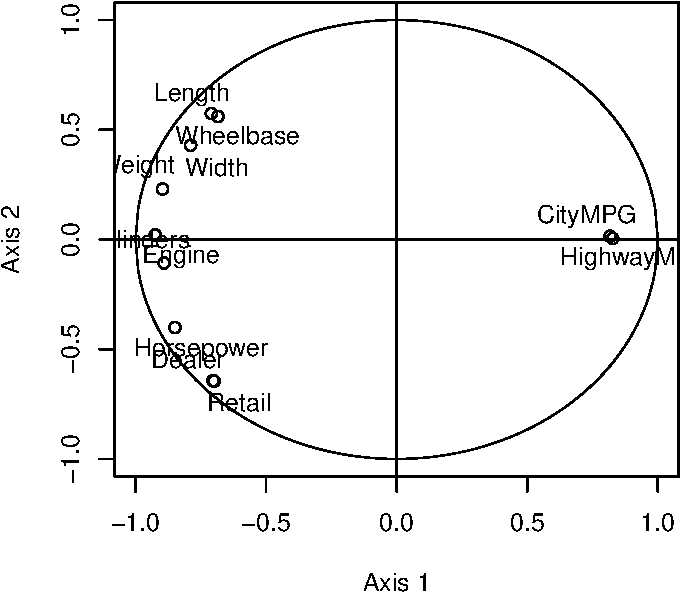
\includegraphics{TD-PCA-correc_files/figure-latex/unnamed-chunk-7-1} \end{center}
     \caption{Variable space}
     \label{fig:cars04:PCA:variable}
  \end{subfigure}
  \hspace{5pt}
  \begin{subfigure}[b]{0.47\textwidth}

\begin{center}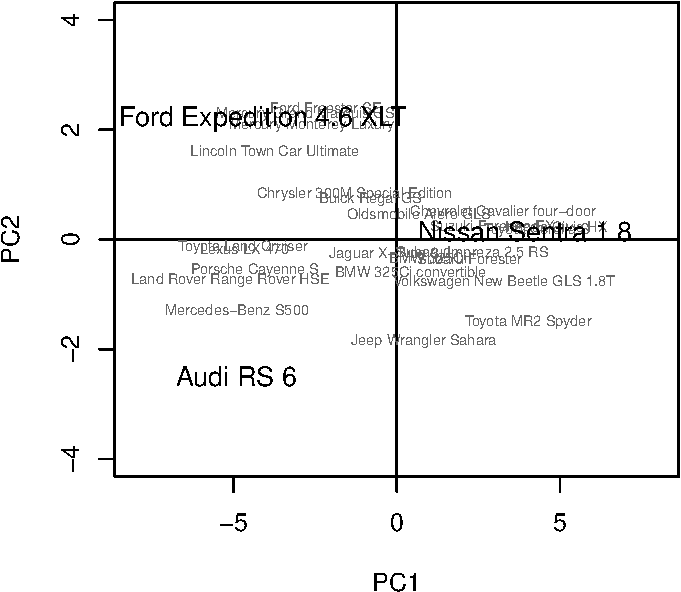
\includegraphics{TD-PCA-correc_files/figure-latex/unnamed-chunk-8-1} \end{center}
    \caption{Individual space}
     \label{fig:cars04:PCA:individual}
  \end{subfigure}
\caption{Principal component representation in the first plane of the variable and of the sample spaces.}
  \label{fig:cars04:PCA}
\end{figure}

\hypertarget{exercise-3}{%
\section{Exercise 3}\label{exercise-3}}

Correspondence Analysis (CA) is an adaptation of PCA to study couples of
qualitative variables. Let consider a couple of qualitative variables
\((X,Y)\) observed on \(n\) samples. The observations are denoted
\(((x_1,y_1),\ldots,(x_n,y_n))\). Two PCAs will be performed.

\begin{itemize}
\item
The first PCA considers the labels $i$ of $X$ as individuals. 
Each individual is described by  conditional frequencies
$f(Y=1 | X=i),\ldots,f(Y=L | X=i)$ of values $j$ of the variable $Y$ given 
$X=i$. 
\item
The second PCA considers the labels $j$ of $Y$ as individuals. 
Each individual is now  characterized by conditional frequencies 
$f(X=1 | Y=j),\ldots,f(X=K | Y=j)$. 
\end{itemize}

The interpretations of these two PCAs can be done as usual. The
advantage of CA is its ability to represent both PCAs on the same graph.
It allows to associate the values \(i\) of \(X\) with values \(j\) of
\(Y\) using inner product between these two vectors.

\begin{itemize}
\item
If the inner product is positive, it means that  $(X=i, Y=j)$ is more frequent in 
the population than it would be under independence between $X$ and $Y$. 
\item
If the value is negative, it means that we would expect more couples $(X=i, Y=j)$ 
under independence property.
\end{itemize}

We propose to apply CA on results recorded after the first turn of
presidential election in France in 2017. \(X\) represent the candidates
and \(Y\) the overseas departments. Interpret the CA results.

N.B.
\textit{Candidate Lassalle was removed because he obtained quite small percentages of votes 
but with a very high relative variability.}

\begin{figure}[htp]
  \centering
  \begin{subfigure}[b]{0.47\textwidth}
    \includegraphics{img/elec2017_afc12_z}
     \caption{PCA on samples: Departments and  candidates (axes 1 and 2)}
     \label{fig:elec2017:axis12}
  \end{subfigure}
  \hspace{5pt}
  \begin{subfigure}[b]{0.47\textwidth}
    \includegraphics{img/elec2017_afc13_z}
    \caption{PCA on samples: Departments and  candidates (axes 1 and 3)}
     \label{fig:elec2017:axis13}
  \end{subfigure}
  \begin{subfigure}[b]{0.47\textwidth}
    \includegraphics{img/elec2017_afc12_var_z}
     \caption{PCA on candidates considered as variables (axes 1 and 2)}
     \label{fig:elec2017:axis12:var}
  \end{subfigure}
  \hspace{5pt}
  \begin{subfigure}[b]{0.47\textwidth}
    \includegraphics{img/elec2017_afc13_var_z}
    \caption{PCA on candidates considered as variables (axes 1 and 3)}
     \label{fig:elec2017:axis13:var}
  \end{subfigure}
  \caption{Principal axes of the two PCA}
\end{figure}

\hypertarget{exercise-4}{%
\section{Exercise 4}\label{exercise-4}}

\begin{enumerate}
\item Prove Proposition \ref{theo:inertia_projection}. 
\begin{proposition}
    Let $x^\prime_i = x_i - {\bar x}_i$ (for $i=1,\ldots,n$) be some centred sample in dimension $p$ with covariance matrix~$\Sigma$. Then the canonical inertia of these points ${\displaystyle{\frac{1}{n}\sum\limits_{i=1}^n \|x^\prime_i\|^2}}$ is ${\mbox{tr}}(\Sigma)$.\\
    Let $\Pi$ some orthogonal projection (with the canonical dot product). Then the inertia of the projected points is ${\mbox{tr}}(\Sigma \Pi)$.
    \label{theo:inertia_projection}
\end{proposition}
\item As a bonus, prove its Corollaries.
\begin{corollary}
    As a consequence, for standardized samples, ${\displaystyle{\frac{1}{n}\sum\limits_{i=1}^n \|x^\prime_i\|^2}} = p$.
\end{corollary} 
\begin{corollary}
    The projected inertia on the sum of two orthogonal subspaces is the sum of the projected inertia on each subspace.
\end{corollary} 
Hint: for any $a \in \R,\, a = {\mbox{tr}}(a)$.
\end{enumerate}

\hypertarget{exercise-5}{%
\section{Exercise 5}\label{exercise-5}}

\begin{enumerate}
\item Prove Proposition \ref{theo:inertia_optimization}. 
\begin{proposition}
        We use the notations in Proposition \ref{theo:inertia_projection}.\\
        Let $a_1$ some vector with norm 1 such that $\Sigma a_1 = \lambda_1 a_1$, $\lambda_1$ being (one of) the highest eigenvalue of $\Sigma$. Then the projected inertia on the line $D_1={\mbox{Span}}(a_1)$ is maximal over projected inertia on all other possible lines. \\
        Moreover, the projected inertia on $D_1$ is $\lambda_1$.    
    \label{theo:inertia_optimization}       
\end{proposition}
\end{enumerate}

Hints:

\begin{itemize}
    \item Use the results from multiple linear regression to prove that for any matrix $X$ with linearly independent columns $X^{(1)},\ldots, X^{(p)}$, the matrix of the orthogonal projection on ${\mbox{Span}}\left(\left\lbrace X^{(1)},\ldots, X^{(p)}\right\rbrace\right)$ is $X (X^T X)^{-1} X^T$ (or admit this result if it does not seem obvious).
    \item Write the maximization problem as 
    $$
    \max\limits_{a, \|a\|=1} {\mbox{tr}}(\Sigma a a^T).
    $$
    \item Introduce a Lagrange multiplier $\xi$ and cancel the gradient of 
    $$
    (a, \xi) \rightarrow a^T \Sigma a - \xi (a^T a-1).
    $$
    \end{itemize}

\end{document}
